\chapter{Results}
This chapter presents the experimental results and analysis of the pix2pix model. Both quantitative and qualitative evaluations are provided to assess its performance under different training configurations. The primary objective is to verify the model’s effectiveness in reconstructing the full-spectrum band and to understand how various factors—such as the amount of training data, the inclusion of specific spectral bands, and the incorporation of different loss functions—affect the final outcomes.

Because GAN-based models require extensive hyperparameter tuning and experimentation, numerous trials were conducted to determine the optimal configuration that stabilizes training, mitigates model collapse, accelerates convergence, and ensures high image quality. These preliminary experiments were initially performed on 20\% of the winter subset to efficiently explore different setups. However, the results obtained with this limited data were unsatisfactory. Following the hypothesis that training on a larger dataset would enhance performance, the model was subsequently trained on the entire winter subset, consisting of 31,825 image pairs.

Finally, a series of ablation studies were performed to analyze the contribution of individual components. Specifically, the experiments investigated (i) the effect of incorporating different loss functions during training and (ii) the impact of excluding the 60 m resolution bands from the input features. These studies provide deeper insight into the model’s data dependency, the role of spectral information, and the influence of various loss terms on reconstruction quality.

The remainder of this chapter is organized as follows. Section 2 presents the results from training on 20\% of the dataset, while Section 3 reports the outcomes from the full winter subset. Section 4 covers ablation studies on loss functions and input bands, and Section 5 summarizes the main findings.

\section{Results on 20\% of the Dataset}
In the initial stage of experimentation, only 20\% of the data were used for training. From the 31,825 image pairs in the winter subset, 3,215, 981, and 981 pairs were allocated for training, validation, and testing, respectively. The model was trained to reconstruct the full optical spectrum consisting of 13 bands, using the dual VV and VH polarization SAR data as input.

The preprocessing steps, training pipeline, and hyperparameter settings were identical to those described previously and were applied unchanged to the experiments on the full winter subset. Moreover, the training was conducted using the full combination of loss functions, as discussed in Section~\ref{subsec:losses}.
\textcolor{red}{report SSIM in mean not median}
\begin{table}[h!]
\centering
\caption[Quantitative results of 20\% training winter subset]{Quantitative results of the training on 20\% of the winter subset.}
\begin{tabular}{lccccc}
\toprule
\textbf{SSIM} & \textbf{PSNR (dB)} & \textbf{LPIPS} & \textbf{SAM (°)} & \textbf{MAE} & \textbf{RMSE} \\
\midrule
0.859 & 27.65 & 0.224 & 6.71 & 195.30 & 381.57 \\
\bottomrule
\end{tabular}
\label{tab:quantitative_result_20}
\end{table}

As shown in Table~\ref{tab:quantitative_result_20}, the model performance is semi-okay, the results are comparable with the state-of-the-art. 
\textcolor{red}{compare against sota}

Examining the qualitative results in Figure~\ref{fig:qualitative_results_20}, the model successfully captures large-scale structural patterns such as boundaries, edges, and terrain formations. However, it struggles to reproduce fine-grained details and textural content. For instance, in row~(a), the boundaries of the agricultural fields are well preserved, but the internal texture of the fields is poorly reconstructed. Similarly, in row~(b), the terrain structure is correctly represented, yet the elevation contrast and depth variation are not accurately reproduced. In row~(c), the coastline and water boundaries are distinctly captured, whereas the urban area in the bottom-right corner appears blurred and lacks definition. Lastly, in row~(d), since the corresponding SAR input contains limited structural information, the generated optical output deviates substantially from the ground truth, indicating the model’s reduced ability to infer fine details in textureless regions.

Overall, these observations confirm that while the \textit{pix2pix} model learns global spatial correspondences effectively, its ability to synthesize fine textures remains limited, particularly in homogeneous or low-contrast regions of the SAR input. Moreover, the inherent differences in imaging principles and physical characteristics between SAR and optical data further challenge the model’s capacity to reconstruct fine spatial and spectral details. Motivated by these findings, the hypothesis was formulated that the model’s performance could be improved by training on a larger-scale dataset. To test this hypothesis, the model was subsequently trained on the full winter subset, and the corresponding results are discussed in the following section.

\begin{figure}[h!]
    \centering
    \setlength{\tabcolsep}{2pt} % horizontal padding between columns (same as ablation)
    \renewcommand{\arraystretch}{1.0} % vertical padding (same as ablation)

    \begin{tabular}{c *{3}{c}}
        % ------------------- Row 1 -------------------
        \textbf{(a)} &
        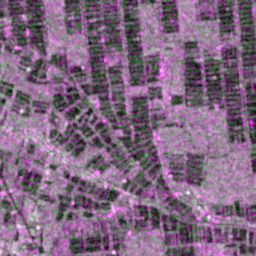
\includegraphics[width=0.2\textwidth, height=0.2\textheight, keepaspectratio]{img/qualitative-20/sample_1/sar.png} &
        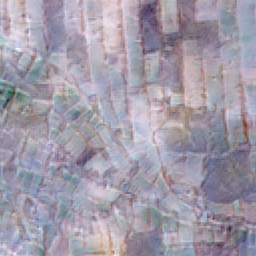
\includegraphics[width=0.2\textwidth, height=0.2\textheight, keepaspectratio]{img/qualitative-20/sample_1/gen.png} &
        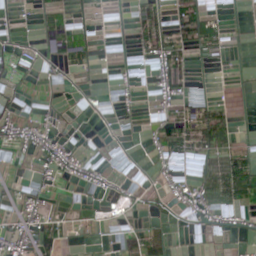
\includegraphics[width=0.2\textwidth, height=0.2\textheight, keepaspectratio]{img/qualitative-20/sample_1/gt.png} \\
        % ------------------- Row 2 -------------------
        \textbf{(b)} &
        \includegraphics[width=0.2\textwidth, height=0.2\textheight, keepaspectratio]{img/qualitative-20/sample_3/sar.png} &
        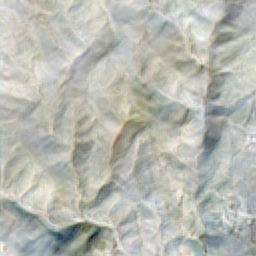
\includegraphics[width=0.2\textwidth, height=0.2\textheight, keepaspectratio]{img/qualitative-20/sample_3/gen.png} &
        \includegraphics[width=0.2\textwidth, height=0.2\textheight, keepaspectratio]{img/qualitative-20/sample_3/gt.png} \\
        \textbf{(c)} &
        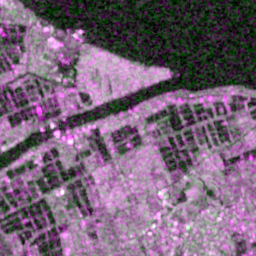
\includegraphics[width=0.2\textwidth, height=0.2\textheight, keepaspectratio]{img/qualitative-20/sample_5/sar.png} &
        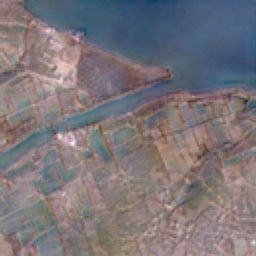
\includegraphics[width=0.2\textwidth, height=0.2\textheight, keepaspectratio]{img/qualitative-20/sample_5/gen.png} &
        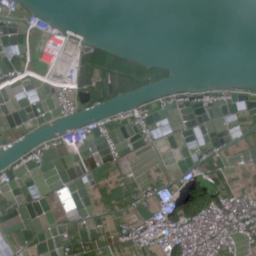
\includegraphics[width=0.2\textwidth, height=0.2\textheight, keepaspectratio]{img/qualitative-20/sample_5/gt.png} \\
        % ------------------- Row 6 -------------------
        \textbf{(d)} &
        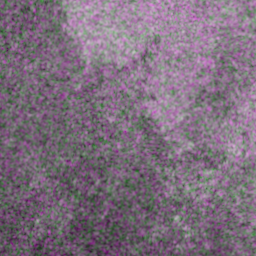
\includegraphics[width=0.2\textwidth, height=0.2\textheight, keepaspectratio]{img/qualitative-20/sample_7/sar.png} &
        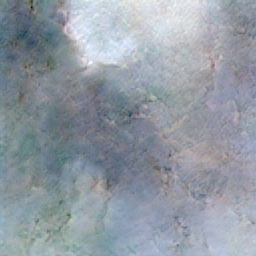
\includegraphics[width=0.2\textwidth, height=0.2\textheight, keepaspectratio]{img/qualitative-20/sample_7/gen.png} &
        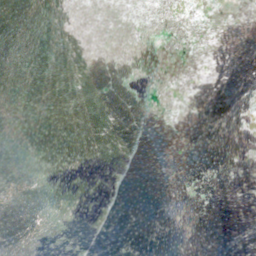
\includegraphics[width=0.2\textwidth, height=0.2\textheight, keepaspectratio]{img/qualitative-20/sample_7/gt.png} \\
    \end{tabular}

    \caption[Qualitative results of 20\% training winter subset]{%
    Qualitative comparison showing representative SAR-to-optical translation results (rows). Columns: 
    \textbf{(i)}~SAR input (pseudo RGB), 
    \textbf{(ii)}~model-generated optical image, 
    \textbf{(iii)}~ground-truth Sentinel-2 image (RGB).
    }
    \label{fig:qualitative_results_20}
\end{figure}

\section{Results on the Full Winter Subset}
GAN-based models generally require large amounts of training data to achieve high-quality image generation, particularly when using mono-temporal SAR imagery as input for translation to optical domains~\cite{sar_2_opt_CGAN_survey_taxonomy}, and especially when reconstructing the full spectral range. Since training on only 20\% of the dataset did not yield satisfactory results, an additional experiment was conducted using the full winter subset, which comprises 31,825 samples divided in an 8:1:1 ratio for training, validation, and testing. This corresponds to approximately 25,460 samples for training and 3,180 samples each for validation and testing. The data preprocessing procedure, training pipeline, and hyperparameters were kept identical to those used in the 20\% experiment to ensure that the effect of training data size was isolated and directly evaluated.

The model required approximately 25$\sim$hours to complete 150~epochs of training. The experimental hypothesis was confirmed: increasing the size of the training dataset led to a clear improvement in model performance. As shown in Table~\ref{tab:quantitative_result_scale}, expanding the training data from 20\% to the full winter subset resulted in substantial gains across all evaluation metrics. In particular, the LPIPS score decreased from 0.224 to 0.173, indicating that the model trained on the full dataset produced outputs with higher perceptual similarity to the ground truth. Likewise, the median SAM value dropped from 6.71° to 4.41°, demonstrating a notable enhancement in spectral consistency across all bands. Furthermore, PSNR increased by approximately 5$\sim$dB, while MAE and RMSE decreased by more than 25\%, confirming the strong positive effect of data scale on reconstruction quality.

\begin{table}[h!]
    \centering
    \caption[Quantitative results for different training data scales: 20\% \& 100\%]{Quantitative results of training on 20\% and 100\% of the winter subset. Arrows ($\uparrow$ / $\downarrow$) indicate whether higher or lower values denote better performance, respectively.}
    \begin{tabular}{lcccccc}
        \toprule
        \textbf{Training Data} & \textbf{SSIM $\uparrow$} & \textbf{PSNR (dB) $\uparrow$} & \textbf{LPIPS $\downarrow$} & \textbf{SAM (°) $\downarrow$} & \textbf{MAE $\downarrow$} & \textbf{RMSE $\downarrow$} \\
        \midrule
        20\% of subset         & 0.859                    & 27.65                         & 0.224                       & 6.71                          & 195.30                    & 381.57                     \\
        100\% of subset        & \textbf{0.888}           & \textbf{32.63}                & \textbf{0.173}              & \textbf{4.41}                 & \textbf{140.72}           & \textbf{233.69}            \\
        \bottomrule
    \end{tabular}
    \label{tab:quantitative_result_scale}
\end{table} 
Similarly, the image reconstruction quality improves noticeably with a larger training dataset. Qualitative examples are shown in Figure~\ref{fig:qualitative_results_100_20}. The model trained on the full winter subset not only better preserves the structural details of the reference images but also achieves markedly enhanced color fidelity, as evident in column (a). In the urban scene (b), it accurately reconstructs the city layout and successfully delineates the river traversing the area. Furthermore, compared to the model trained on only 20\% of the data, the full-data model better captures surface relief and elevation depth, as illustrated in (c).

These qualitative and quantitative improvements demonstrate that increasing the amount and diversity of training data enables the model to more effectively learn both the perceptual and spectral characteristics of the optical domain, ultimately guiding it toward more realistic and color-consistent reconstructions.

\begin{figure}[h!]
    \centering
    \setlength{\tabcolsep}{2pt} % horizontal padding between columns (same as ablation)
    \renewcommand{\arraystretch}{1.0} % vertical padding (same as ablation)

    \begin{tabular}{c *{4}{c}}
        % ------------------- Row 1 -------------------
        \textbf{(a)} &
        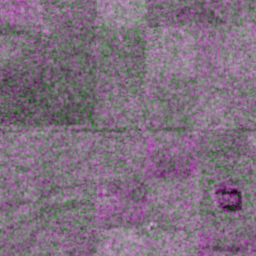
\includegraphics[width=0.2\textwidth, height=0.2\textheight, keepaspectratio]{img/qualitative-20-full/sample_1/sar.png} &
        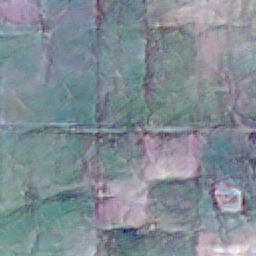
\includegraphics[width=0.2\textwidth, height=0.2\textheight, keepaspectratio]{img/qualitative-20-full/sample_1/gen_0.2.png} &
        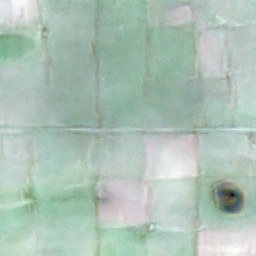
\includegraphics[width=0.2\textwidth, height=0.2\textheight, keepaspectratio]{img/qualitative-20-full/sample_1/gen_full.png} &
        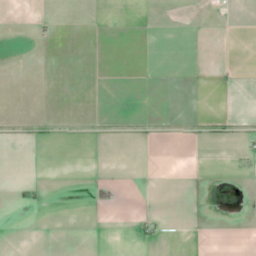
\includegraphics[width=0.2\textwidth, height=0.2\textheight, keepaspectratio]{img/qualitative-20-full/sample_1/gt.png} \\
        % ------------------- Row 2 -------------------
        \textbf{(b)} &
        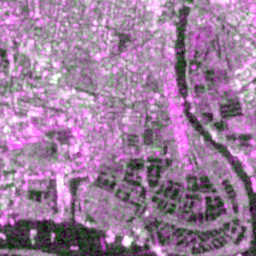
\includegraphics[width=0.2\textwidth, height=0.2\textheight, keepaspectratio]{img/qualitative-20-full/sample_2/sar.png} &
        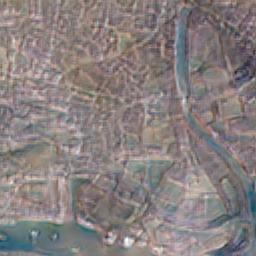
\includegraphics[width=0.2\textwidth, height=0.2\textheight, keepaspectratio]{img/qualitative-20-full/sample_2/gen_0.2.png} &
        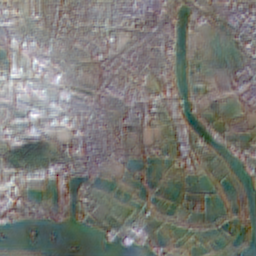
\includegraphics[width=0.2\textwidth, height=0.2\textheight, keepaspectratio]{img/qualitative-20-full/sample_2/gen_full.png} &
        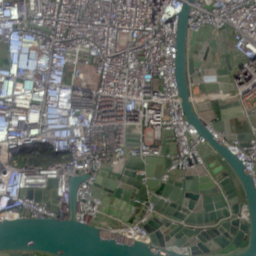
\includegraphics[width=0.2\textwidth, height=0.2\textheight, keepaspectratio]{img/qualitative-20-full/sample_2/gt.png} \\
        \textbf{(c)} &
        \includegraphics[width=0.2\textwidth, height=0.2\textheight, keepaspectratio]{img/qualitative-20-full/sample_3/sar.png} &
        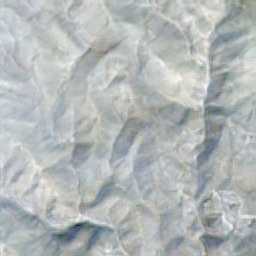
\includegraphics[width=0.2\textwidth, height=0.2\textheight, keepaspectratio]{img/qualitative-20-full/sample_3/gen_0.2.png} &
        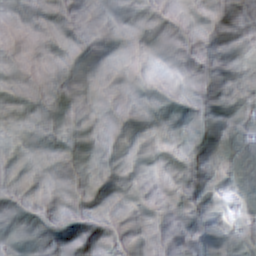
\includegraphics[width=0.2\textwidth, height=0.2\textheight, keepaspectratio]{img/qualitative-20-full/sample_3/gen_full.png} &
        \includegraphics[width=0.2\textwidth, height=0.2\textheight, keepaspectratio]{img/qualitative-20-full/sample_3/gt.png} \\
        % ------------------- Row 6 -------------------
        \textbf{(d)} &
        \includegraphics[width=0.2\textwidth, height=0.2\textheight, keepaspectratio]{img/qualitative-20-full/sample_4/sar.png} &
        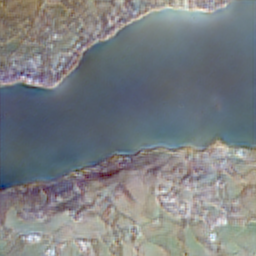
\includegraphics[width=0.2\textwidth, height=0.2\textheight, keepaspectratio]{img/qualitative-20-full/sample_4/gen_0.2.png} &
        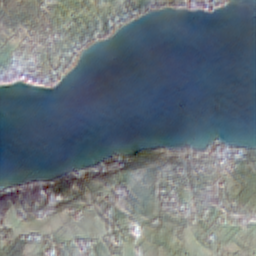
\includegraphics[width=0.2\textwidth, height=0.2\textheight, keepaspectratio]{img/qualitative-20-full/sample_4/gen_full.png} &
        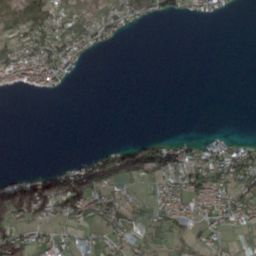
\includegraphics[width=0.2\textwidth, height=0.2\textheight, keepaspectratio]{img/qualitative-20-full/sample_4/gt.png} \\
    \end{tabular}

    \caption[Qualitative results for different training data scales: 20\% \& 100\%]{%
    Qualitative comparison of models trained on 20\% and 100\% of the dataset. 
    Columns: \textbf{(i)}~SAR input (pseudo-RGB), 
    \textbf{(ii)}~generated optical image from 20\% training, 
    \textbf{(iii)}~generated optical image from 100\% training, and 
    \textbf{(iv)}~ground-truth Sentinel-2 image. All optical images are depicted in RGB (B4, B4, B2) batch.}
    \label{fig:qualitative_results_100_20}
\end{figure}

\section{Results Across Individual Optical Bands}
Another objective of this work was to assess the model’s ability to reliably reconstruct each optical band individually and to evaluate the extent of its accuracy across the spectrum. 
For this purpose, the model trained on the full winter subset was evaluated separately for all Sentinel-2 bands, and the corresponding results are summarized in Table~\ref{tab:per_band_validation}.

When comparing the reconstruction quality across individual bands, the focus is placed on the unitless SSIM metric. Other metrics such as MAE or RMSE are not directly comparable between bands, as they depend on the absolute magnitude and statistical distribution of reflectance values, which differ across spectral ranges. In contrast, SSIM measures local structural similarity based on relative intensity patterns rather than absolute values. While not entirely invariant to scale differences, SSIM provides a more robust and interpretable basis for cross-band comparison in this context.

\begin{table}[h!]
\centering
\caption[Per-band validation results for full dataset training]{%
Per-band quantitative validation results of the \textit{pix2pix} model trained on the full winter subset. Each Sentinel-2 band’s central wavelength, spectral designation, and native spatial resolution are listed for reference.}
\resizebox{0.9\textwidth}{!}{%
\begin{tabular}{lcccc}
\toprule
\textbf{Band} & \textbf{PSNR (dB) $\uparrow$} & \textbf{SSIM $\uparrow$} & \textbf{Central Wavelength [nm]} & \textbf{Spectral / Resolution [m]} \\
\midrule
B1   &  36.53  &  0.9758 & 443  & Aerosols / 60 \\
B2   &  37.49  &  0.9506 & 490  & Blue / 10 \\
B3   &  35.67  &  0.9199 & 560  & Green / 10 \\
B4   &  32.84  &  0.8639 & 665  & Red / 10 \\
B5   &  33.68  &  0.9007 & 705  & Red Edge / 20 \\
B6   &  31.62  &  0.8536 & 740  & Red Edge / 20 \\
B7   &  30.37  &  0.8253 & 783  & Red Edge / 20 \\
B8   &  29.62  &  0.7738 & 842  & NIR / 10 \\
B8A  &  29.62  &  0.8071 & 865  & Red Edge / 20 \\
B9   &  33.99  &  0.9388 & 945  & Water Vapour / 60 \\
B10  &  32.12  &  0.9386 & 1375 & Cirrus / 60 \\
B11  &  29.92  &  0.8309 & 1610 & SWIR / 20 \\
B12  &  31.48  &  0.8586 & 2190 & SWIR / 20 \\
\bottomrule
\end{tabular}% 
}
\label{tab:per_band_validation}
\end{table}

Notably, Band~8 (NIR), despite its native spatial resolution of 10~m, exhibits the lowest reconstruction performance among all bands, including those at coarser resolutions, as illustrated in Figure~\ref{fig:ssim_per_band}. This suggests a weaker correlation between SAR backscatter and NIR reflectance compared to other spectral regions, likely due to their differing sensitivity to surface structure and vegetation properties. In contrast, the 60~m atmospheric correction bands—B1 (Aerosols), B9 (Water Vapour), and B10 (Cirrus)—are reconstructed reliably, with B1 achieving the highest SSIM overall. Their smoother spectral characteristics and lower spatial variability likely facilitate more stable and accurate predictions, even after resampling to 10 m.

\begin{figure}[h!]
\centering
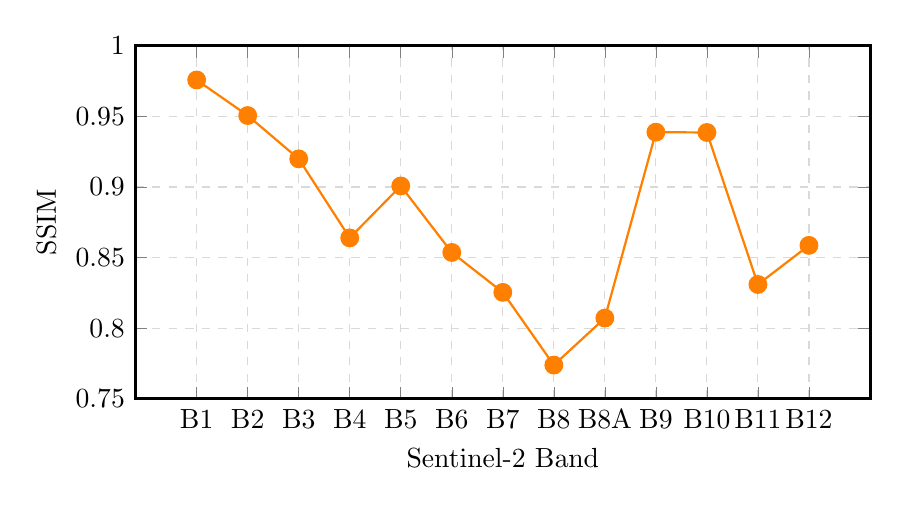
\begin{tikzpicture}
\begin{axis}[
    width=0.9\textwidth,
    height=0.5\textwidth,
    xlabel={Sentinel-2 Band},
    ylabel={SSIM},
    ymin=0.75, ymax=1.0,
    ytick distance=0.05,
    xtick=data,
    xticklabels={B1,B2,B3,B4,B5,B6,B7,B8,B8A,B9,B10,B11,B12},
    grid=major,
    grid style={dashed,gray!30},
    every axis plot/.append style={thick, mark=*},
    mark size=3pt,
    line width=1pt,
]

\addplot[
    color=orange,
    mark=*,
    mark options={fill=orange},
]
coordinates {
    (1,0.9758)
    (2,0.9506)
    (3,0.9199)
    (4,0.8639)
    (5,0.9007)
    (6,0.8536)
    (7,0.8253)
    (8,0.7738)
    (9,0.8071)
    (10,0.9388)
    (11,0.9386)
    (12,0.8309)
    (13,0.8586)
};

\end{axis}
\end{tikzpicture}
\caption[Per-band SSIM for the Pix2Pix model]{Per-band SSIM for the \textit{pix2pix} model trained on the full winter subset.}
\label{fig:ssim_per_band}
\end{figure}

To visually complement the quantitative assessment, representative grayscale examples for each Sentinel-2 band are provided in Appendix~\ref{appendix:bandwise_results}. Each example illustrates the generated band alongside its corresponding ground-truth reference, enabling a direct visual evaluation of the reconstruction quality and spatial consistency across the spectrum.

\newpage

\section{Ablation Studies}
\subsection{Effect of Loss Functions}
\label{subsec:ablation_loss}

To evaluate the contribution of each loss component to the overall model performance, an ablation study was conducted. Four training configurations were compared:
\begin{enumerate}
    \item $\mathcal{L}_{\text{GAN}} + \mathcal{L}_{\text{L1}}$,
    \item $\mathcal{L}_{\text{GAN}} + \mathcal{L}_{\text{L1}} + \mathcal{L}_{\text{SSIM}}$,
    \item $\mathcal{L}_{\text{GAN}} + \mathcal{L}_{\text{L1}} + \mathcal{L}_{\text{LPIPS}}$, and
    \item the full combination $\mathcal{L}_{\text{GAN}} + \mathcal{L}_{\text{L1}} + \mathcal{L}_{\text{SSIM}} + \mathcal{L}_{\text{LPIPS}}$.
\end{enumerate}
This analysis aimed to isolate the contribution of each additional loss term to both quantitative performance and visual reconstruction quality. The evaluation was conducted using the same IQA metrics employed throughout the thesis, namely SSIM, PSNR, LPIPS, SAM, MAE, and RMSE. Several training loops were conducted using the same preprocessing procedure described in Section~\ref{subsec:preprocessing}. All models were trained under identical settings, hyperparameters, datasets, and number of epochs to ensure a fair and consistent comparison across the different loss configurations.

Table~\ref{tab:ablation_quantitative} summarizes the quantitative performance across the four loss configurations. As shown, the baseline configuration without SSIM and LPIPS achieved the lowest performance across most metrics, with the exception of PSNR. This configuration also represents the weakest setup in terms of overall image quality. As illustrated in Figure~\ref{fig:ablation_samples}(b), images generated by the baseline model differ significantly from the ground truth, both texturally and perceptually. 

\begin{table}[h!]
    \centering
    \resizebox{\textwidth}{!}{%
        \begin{tabular}{lcccccc}
            \toprule
            \textbf{Loss Configuration}                                                                                   & \textbf{SSIM $\uparrow$} & \textbf{PSNR (dB) $\uparrow$} & \textbf{LPIPS $\downarrow$} & \textbf{SAM~(°) $\downarrow$} & \textbf{MAE $\downarrow$} & \textbf{RMSE $\downarrow$} \\
            \midrule
            $\mathcal{L}_{\text{GAN}} + \mathcal{L}_{\text{L1}}$                                                          & 0.820                    & 26.38                         & 0.287                       & 6.47                          & 229                       & 441                        \\
            $\mathcal{L}_{\text{GAN}} + \mathcal{L}_{\text{L1}} + \mathcal{L}_{\text{SSIM}}$                              & \textbf{0.862}           & \textbf{27.67}                & 0.399                       & \textbf{5.43}                 & 198                       & \textbf{380}               \\
            $\mathcal{L}_{\text{GAN}} + \mathcal{L}_{\text{L1}} + \mathcal{L}_{\text{LPIPS}}$                             & 0.842                    & 27.58                         & \textbf{0.213}              & 5.73                          & 201                       & 385                        \\
            $\mathcal{L}_{\text{GAN}} + \mathcal{L}_{\text{L1}} + \mathcal{L}_{\text{SSIM}} + \mathcal{L}_{\text{LPIPS}}$ & 0.859                    & 27.65                         & 0.224                       & 5.44                          & \textbf{195}              & 382                        \\
            \bottomrule
        \end{tabular}%
    }
    \caption[Quantitative ablation study across loss configurations]{Quantitative results of the ablation study across different loss configurations. Best values per metric are shown in bold.}
    \label{tab:ablation_quantitative}
\end{table}

Notably, integrating SSIM alone yielded the highest quantitative scores in several metrics. However, the qualitative results under this configuration reveal perceptual inconsistencies and reduced visual realism. This discrepancy arises because SSIM does not always align with human perceptual judgments of image similarity. As reported by NVIDIA in~\cite{nvidia_Understanding_SSIM}, SSIM can overemphasize small intensity variations in dark regions, overlook significant color shifts, and assign high similarity near edges even when visible artifacts are present.

\begin{figure}[h!]
    \centering
    \setlength{\tabcolsep}{2pt} % horizontal padding between columns
    \renewcommand{\arraystretch}{1.0} % vertical padding

    % Adjust width so that 6 images fit one row across the text width
    % (tweak 0.155\textwidth to 0.158 or 0.152 if needed)
    \begin{tabular}{*{6}{c}}
        % \toprule
        (a) & (b) & (c) & (d) & (e) & (f) \\
        % \midrule

        % ------------------- Row 1 -------------------
        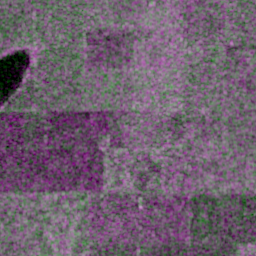
\includegraphics[width=0.155\textwidth]{img/ablation/sample_1/sar.png}   &
        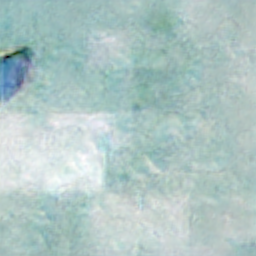
\includegraphics[width=0.155\textwidth]{img/ablation/sample_1/none.png}  &
        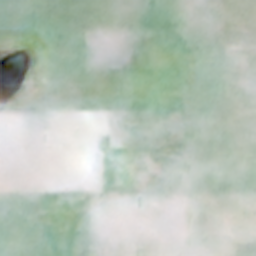
\includegraphics[width=0.155\textwidth]{img/ablation/sample_1/ssim.png}  &
        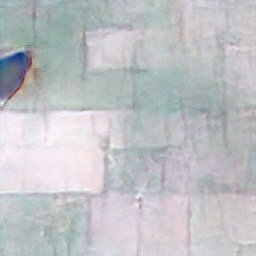
\includegraphics[width=0.155\textwidth]{img/ablation/sample_1/lpips.png} &
        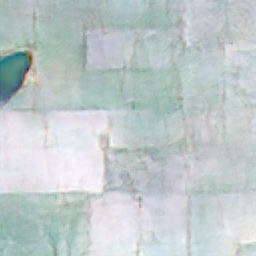
\includegraphics[width=0.155\textwidth]{img/ablation/sample_1/all.png}   &
        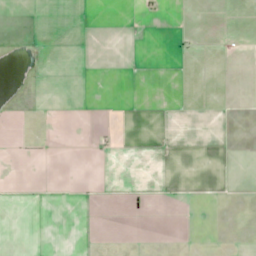
\includegraphics[width=0.155\textwidth]{img/ablation/sample_1/gt.png}                                  \\
        % ------------------- Row 2 -------------------
        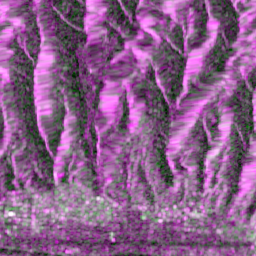
\includegraphics[width=0.155\textwidth]{img/ablation/sample_2/sar.png}   &
        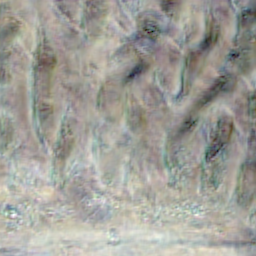
\includegraphics[width=0.155\textwidth]{img/ablation/sample_2/none.png}  &
        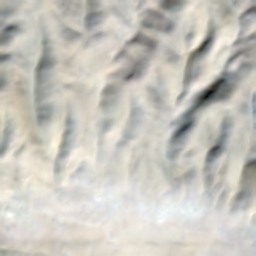
\includegraphics[width=0.155\textwidth]{img/ablation/sample_2/ssim.png}  &
        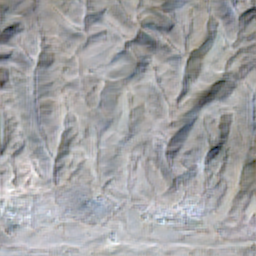
\includegraphics[width=0.155\textwidth]{img/ablation/sample_2/lpips.png} &
        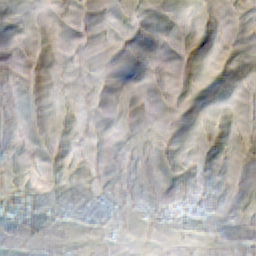
\includegraphics[width=0.155\textwidth]{img/ablation/sample_2/all.png}   &
        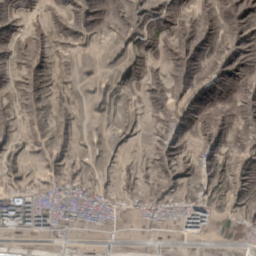
\includegraphics[width=0.155\textwidth]{img/ablation/sample_2/gt.png}                                  \\
        % ------------------- Row 3 -------------------
        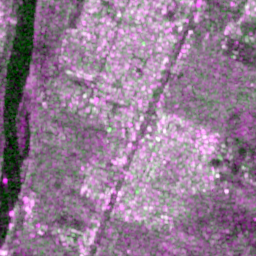
\includegraphics[width=0.155\textwidth]{img/ablation/sample_3/sar.png}   &
        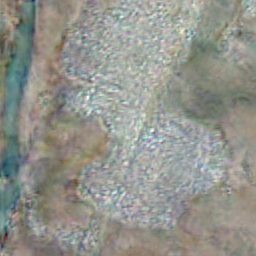
\includegraphics[width=0.155\textwidth]{img/ablation/sample_3/none.png}  &
        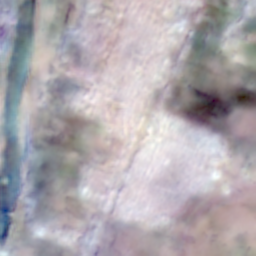
\includegraphics[width=0.155\textwidth]{img/ablation/sample_3/ssim.png}  &
        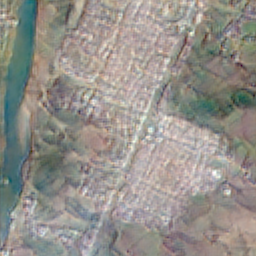
\includegraphics[width=0.155\textwidth]{img/ablation/sample_3/lpips.png} &
        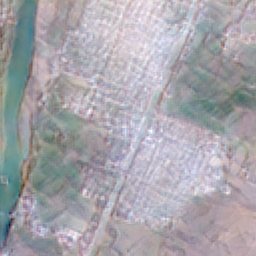
\includegraphics[width=0.155\textwidth]{img/ablation/sample_3/all.png}   &
        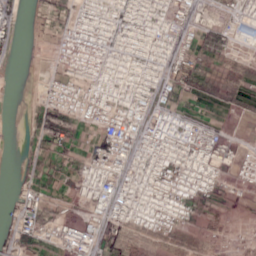
\includegraphics[width=0.155\textwidth]{img/ablation/sample_3/gt.png}                                  \\
        % ------------------- Row 4 -------------------
        \includegraphics[width=0.155\textwidth]{img/ablation/sample_4/sar.png}   &
        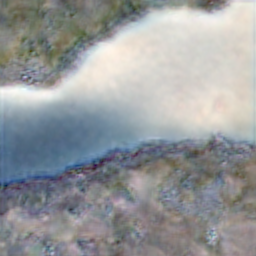
\includegraphics[width=0.155\textwidth]{img/ablation/sample_4/none.png}  &
        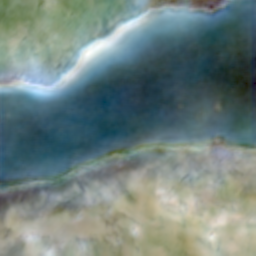
\includegraphics[width=0.155\textwidth]{img/ablation/sample_4/ssim.png}  &
        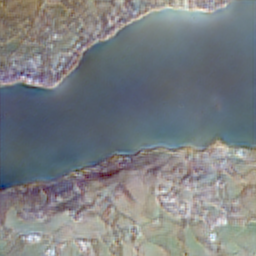
\includegraphics[width=0.155\textwidth]{img/ablation/sample_4/lpips.png} &
        \includegraphics[width=0.155\textwidth]{img/ablation/sample_4/all.png}   &
        \includegraphics[width=0.155\textwidth]{img/ablation/sample_4/gt.png}                                  \\
        % \bottomrule
    \end{tabular}

    \caption[Qualitative ablation study across loss configurations]{%
    Qualitative ablation results showing representative samples (rows) under four configurations (columns):\\
    \textbf{(a)}~Input SAR (pseudo RGB)\\
    \textbf{(b)}~$\mathcal{L}_{\text{GAN}}{+}\mathcal{L}_{\text{L1}}$\\
    \textbf{(c)}~$\mathcal{L}_{\text{GAN}}{+}\mathcal{L}_{\text{L1}}{+}\mathcal{L}_{\text{SSIM}}$\\
    \textbf{(d)}~$\mathcal{L}_{\text{GAN}}{+}\mathcal{L}_{\text{L1}}{+}\mathcal{L}_{\text{LPIPS}}$\\
    \textbf{(e)}~all four losses combined\\
    \textbf{(f)}~ground-truth Sentinel-2 optical image (RGB bands).
    }
    \label{fig:ablation_samples}
\end{figure}

Since the primary objective of LPIPS is to measure perceptual similarity, incorporating it into the baseline configuration led to notable improvements in the preservation of low-level features. As illustrated in column~(d) of Figure~\ref{fig:ablation_samples}, the model was able to maintain sharper edges and more distinct boundaries. Moreover, the generated images appear visually more realistic and closely resemble the ground truth in texture and detail. However, the colour reproduction achieved with LPIPS is slightly inferior to that obtained using SSIM, as the SSIM-based model produces more natural and accurate colours overall.

The full combination of all four losses achieved the best balance between pixel-level accuracy, perceptual realism, and structural coherence. 
Its SAM values were the second best, differing only marginally from the SSIM-only configuration. 
By incorporating both SSIM and LPIPS, the model attains an effective balance between color, luminance, and perceptual realism, as shown in column~(e) of Figure~\ref{fig:ablation_samples}. 
Similar findings were also reported by~\cite{s2o_ViT_cGAN} and~\cite{CR_RS_GAN_s2o}. 
 
Overall, the results demonstrate the incremental benefit of incorporating perceptual and structural similarity terms alongside the adversarial $\mathcal{L}_{\text{GAN}}$ and $\mathrm{L1}$ objectives. 

\subsection{Effect of Excluding 60 m Bands}
Given the varying data distributions and the originally different spatial resolutions of the Sentinel-2 bands (even though all were resampled to 10m in the dataset), it was hypothesized that including the 60m bands might introduce noise and confuse the model during training. To examine this assumption, an ablation study was conducted using the same training configuration as for the full 13-band model, both trained on 20\% of the winter subset.

Surprisingly, removing the 60m bands did not lead to any improvement. Instead, both SSIM and LPIPS scores decreased, as reported in Table~\ref{tab:ablation_excluding_60m}. This suggests that the 60m bands, which primarily serve for atmospheric correction (e.g., B1, B9, and B10), provide complementary spectral information that contributes to maintaining spectral fidelity during training.

\begin{table}[h!]
    \centering
    \setlength{\tabcolsep}{8pt}
    \renewcommand{\arraystretch}{1.15}
    \caption[[Overall performance when excluding 60m bands]]{Overall performance comparing all 13 bands vs. excluding the 60m bands (B1, B9, B10).}
    \label{tab:ablation_excluding_60m}
    \begin{tabular}{lccc}
        \hline
        \textbf{Setting} & \textbf{SSIM $\uparrow$} & \textbf{PSNR (dB) $\uparrow$} & \textbf{SAM~(°) $\downarrow$} \\
        \hline
        All 13 bands & 0.859390 & 27.650251 & 6.7064 \\
        Excluding 60m (B1,B9,B10) & 0.825861 & 26.474423 & 6.3339 \\
        \hline
    \end{tabular}
    % Note: SAM is computed in 13-band space for "All 13 bands" and in 10-band space when excluding 60 m bands.
\end{table}

Interestingly, while the SAM slightly improved after excluding the 60m bands, this does not necessarily contradict the decline in PSNR and SSIM. The model may have learned to reproduce more spectrally consistent relationships between the remaining bands (hence a smaller spectral angle), yet failed to preserve the absolute reflectance magnitudes and spatial details, leading to lower overall reconstruction quality. This indicates a trade-off between radiometric fidelity and spectral coherence in the absence of the full spectral range. For qualitative evaluation, Figure~\ref{fig:ablation_excluding_60m_qualitative} illustrates the generated optical images obtained from models trained with the full spectral configuration and with the 60,m bands excluded.

Similarly, the per-band evaluation (Table~\ref{tab:ablation_excluding_60m_per_band}) confirms this trend. For most bands, SSIM remains stable when all bands are included, indicating consistent structural reconstruction quality. However, PSNR decreases for nearly all bands when the 60m bands are excluded, with the exception of B1, demonstrating that the full spectral configuration better supports radiometric reconstruction.
\begin{figure}[h!]
    \centering
    \setlength{\tabcolsep}{2pt} % horizontal padding between columns
    \renewcommand{\arraystretch}{1.0} % vertical padding

    \begin{tabular}{cccc}
        % ------------------- Rows -------------------
        \includegraphics[width=0.2\textwidth, height=0.2\textheight, keepaspectratio]{img/exclusion_60_m/bands10/sample_000034_sar_pseudo.png} &
        \includegraphics[width=0.2\textwidth, height=0.2\textheight, keepaspectratio]{img/exclusion_60_m/bands10/sample_000034_pred_rgb.png} &
        \includegraphics[width=0.2\textwidth, height=0.2\textheight, keepaspectratio]{img/exclusion_60_m/bands13/sample_000034_pred_rgb.png} &
        \includegraphics[width=0.2\textwidth, height=0.2\textheight, keepaspectratio]{img/exclusion_60_m/bands10/sample_000034_true_rgb.png} \\

        \includegraphics[width=0.2\textwidth, height=0.2\textheight, keepaspectratio]{img/exclusion_60_m/bands10/sample_000050_sar_pseudo.png} &
        \includegraphics[width=0.2\textwidth, height=0.2\textheight, keepaspectratio]{img/exclusion_60_m/bands10/sample_000050_pred_rgb.png} &
        \includegraphics[width=0.2\textwidth, height=0.2\textheight, keepaspectratio]{img/exclusion_60_m/bands13/sample_000050_pred_rgb.png} &
        \includegraphics[width=0.2\textwidth, height=0.2\textheight, keepaspectratio]{img/exclusion_60_m/bands10/sample_000050_true_rgb.png} \\

        \includegraphics[width=0.2\textwidth, height=0.2\textheight, keepaspectratio]{img/exclusion_60_m/bands10/sample_000010_sar_pseudo.png} &
        \includegraphics[width=0.2\textwidth, height=0.2\textheight, keepaspectratio]{img/exclusion_60_m/bands10/sample_000010_pred_rgb.png} &
        \includegraphics[width=0.2\textwidth, height=0.2\textheight, keepaspectratio]{img/exclusion_60_m/bands13/sample_000010_pred_rgb.png} &
        \includegraphics[width=0.2\textwidth, height=0.2\textheight, keepaspectratio]{img/exclusion_60_m/bands10/sample_000010_true_rgb.png} \\

        \includegraphics[width=0.2\textwidth, height=0.2\textheight, keepaspectratio]{img/exclusion_60_m/bands10/sample_000065_sar_pseudo.png} &
        \includegraphics[width=0.2\textwidth, height=0.2\textheight, keepaspectratio]{img/exclusion_60_m/bands10/sample_000065_pred_rgb.png} &
        \includegraphics[width=0.2\textwidth, height=0.2\textheight, keepaspectratio]{img/exclusion_60_m/bands13/sample_000065_pred_rgb.png} &
        \includegraphics[width=0.2\textwidth, height=0.2\textheight, keepaspectratio]{img/exclusion_60_m/bands10/sample_000065_true_rgb.png} \\
    \end{tabular}

    \caption[Qualitative results when excluding 60\,m bands]{%
    Qualitative comparison of generated optical images when excluding the 60\,m Sentinel-2 bands. 
    Columns: \textbf{(i)}~SAR input (pseudo-RGB), 
    \textbf{(ii)}~generated optical image trained without the 60\,m bands, 
    \textbf{(iii)}~generated optical image trained with all 13 bands, and 
    \textbf{(iv)}~reference cloud-free Sentinel-2 image. 
    All optical outputs are visualized in RGB composition (B4, B3, B2).}
    \label{fig:ablation_excluding_60m_qualitative}
\end{figure}

\begin{table}[h!]
    \centering
    \setlength{\tabcolsep}{6pt}
    \renewcommand{\arraystretch}{1.15}
    \caption[Per-band performance when excluding 60m bands]{Per-band comparison of SSIM and PSNR. Columns are ordered as SSIM (no 60\,m), SSIM (13), PSNR (no 60\,m), and PSNR (13). A dash indicates the band was excluded in the 60\,m-removed setting.}
    \label{tab:ablation_excluding_60m_per_band}
    \begin{tabular}{lcccc}
        \hline
        Band & SSIM (no 60\,m) $\uparrow$ & SSIM (13) $\uparrow$ & PSNR (no 60\,m) [dB] $\uparrow$ & PSNR (13) [dB] $\uparrow$ \\
        \hline
        B1   & ---    & 0.9634 & ---    & 29.749 \\
        B2   & 0.9431 & 0.9430 & 34.151 & 34.057 \\
        B3   & 0.9064 & 0.9060 & 31.691 & 31.718 \\
        B4   & 0.8348 & 0.8340 & 28.039 & 28.145 \\
        B5   & 0.8707 & 0.8729 & 28.098 & 28.257 \\
        B6   & 0.8199 & 0.8231 & 26.740 & 26.926 \\
        B7   & 0.7890 & 0.7925 & 25.694 & 25.884 \\
        B8   & 0.7375 & 0.7416 & 25.534 & 25.739 \\
        B8A  & 0.7687 & 0.7722 & 25.095 & 25.311 \\
        B9   & ---    & 0.8666 & ---    & 24.617 \\
        B10  & ---    & 0.8826 & ---    & 24.571 \\
        B11  & 0.7774 & 0.7809 & 23.395 & 23.727 \\
        B12  & 0.8034 & 0.8073 & 24.956 & 25.263 \\
        \hline
    \end{tabular}
\end{table}

